\documentclass[aspectratio=169]{beamer}
\usepackage{will_handley_beamer}
\usepackage{title_page}

% Commands
% --------
% - \arxiv{arxiv number}
% - \arxiv{<number>}            arxiv.org/abs/<number>
% - \oldarxiv{<arxiv number>}   arxiv.org/<number>
% - \doi{<doi>}                 doi.org/<doi>
% - \xkcd{<number>}             xkcd.com/<number>
% - \email{<email>}             <<email>>
% - \tthref{<website>}          <website>
% - \av[dist]{<quantity>}       <quantity>_{dist}
% - \student{<name>}{<detail>}{<photo>}

% Talk details
% ------------
\title{Scanning for cosmological tensions
\subtitle{across a DiRAC-enabled grid of models, datasets and samplers}
\date{21\textsuperscript{st} May 2025}

\begin{document}

%%%%%%%%%%%%%%%%%%%%%%%%%%%%%%%%%%%%%%%%%%%%%%%%%%%%%%%%%%%%%%%%%%%%%%%%%%%%%%%
% Title Slide
%%%%%%%%%%%%%%%%%%%%%%%%%%%%%%%%%%%%%%%%%%%%%%%%%%%%%%%%%%%%%%%%%%%%%%%%%%%%%%%
\begin{frame}
    \titlepage
\end{frame}

%%%%%%%%%%%%%%%%%%%%%%%%%%%%%%%%%%%%%%%%%%%%%%%%%%%%%%%%%%%%%%%%%%%%%%%%%%%%%%%
% The Challenge: Cosmological Tensions & Analysis Robustness
%%%%%%%%%%%%%%%%%%%%%%%%%%%%%%%%%%%%%%%%%%%%%%%%%%%%%%%%%%%%%%%%%%%%%%%%%%%%%%%
\begin{frame}
    \frametitle{The Challenge: Cosmological Tensions \& Analysis Robustness}
    \begin{columns}[T]
        \column{0.55\textwidth}
        \begin{itemize}
            \item Precision cosmology has revealed persistent discrepancies in key parameters:
                \begin{itemize}
                    \item $H_0$ (Hubble constant) [\arxiv{1907.10625}]
                    \item $\sigma_8$/$S_8$ (matter clustering) [\arxiv{1610.04606}]
                    \item $\Omega_K$ (spatial curvature) [\arxiv{1908.09139}, \arxiv{1911.02087}]
                \end{itemize}
            \item This underscores the critical importance of robust cosmological analysis.
            \item Key goals:
                \begin{itemize}
                    \item Accurately \textbf{quantifying tensions} between datasets and models.
                    \item Identifying and \textbf{addressing biases}, e.g., $\Lambda$CDM bias from fiducial assumptions in likelihoods.
                \end{itemize}
            \item We need systematic exploration across a wide range of models and datasets to distinguish new physics from systematics.
        \end{itemize}

        \column{0.45\textwidth}
        \begin{figure}
            \centering
            % Figure from ERC Grant, Fig 1
            \includegraphics[width=\columnwidth]{placeholder_COSMOLOGICAL_TENSIONS_H0_S8_OMEGAK.png}
            \caption{Discrepancies in $H_0$, $S_8$ and $\Omega_K$ highlight the challenge. (Figure adapted from \arxiv{1908.09139} and others)}
        \end{figure}
    \end{columns}
\end{frame}

%%%%%%%%%%%%%%%%%%%%%%%%%%%%%%%%%%%%%%%%%%%%%%%%%%%%%%%%%%%%%%%%%%%%%%%%%%%%%%%
% Bayesian Inference Pillars & The Problem of Scale
%%%%%%%%%%%%%%%%%%%%%%%%%%%%%%%%%%%%%%%%%%%%%%%%%%%%%%%%%%%%%%%%%%%%%%%%%%%%%%%
\begin{frame}
    \frametitle{Bayesian Inference Pillars \& The Problem of Scale}
    \begin{columns}[T]
        \column{0.33\textwidth}
        \begin{block}{Parameter Estimation}
            What do data tell us about model parameters?
            \[ \mathcal{P}(\theta|D,M) = \frac{\mathcal{L}(D|\theta,M) \pi(\theta|M)}{\mathcal{Z}(D|M)} \]
        \end{block}
        \column{0.33\textwidth}
        \begin{block}{Model Comparison}
            How much do data support a model? (Occam's Razor \arxiv{2102.11511})
            \[ P(M|D) = \frac{\mathcal{Z}(D|M) P(M)}{P(D)} \]
            Relies on the Bayesian Evidence $\mathcal{Z}$.
        \end{block}
        \column{0.33\textwidth}
        \begin{block}{Tension Quantification}
            Are datasets consistent under a model? [\arxiv{1902.04029}]
            \[ \mathcal{R} = \frac{\mathcal{Z}_{AB}}{\mathcal{Z}_A\mathcal{Z}_\mathcal{B}}, \quad \log \mathcal{S} = \dots  \]
            Also evidence-based.
        \end{block}
    \end{columns}
    \vfill
    \begin{itemize}
        \item Model comparison and tension quantification are computationally hard, especially across many models/datasets.
        \item This necessitates efficient tools and pre-computed resources.
    \end{itemize}
\end{frame}

%%%%%%%%%%%%%%%%%%%%%%%%%%%%%%%%%%%%%%%%%%%%%%%%%%%%%%%%%%%%%%%%%%%%%%%%%%%%%%%
% DiRAC Allocations: Powering the Search
%%%%%%%%%%%%%%%%%%%%%%%%%%%%%%%%%%%%%%%%%%%%%%%%%%%%%%%%%%%%%%%%%%%%%%%%%%%%%%%
\begin{frame}
    \frametitle{DiRAC Allocations: Powering the Systematic Search}
    \begin{columns}[T]
        \column{0.55\textwidth}
        \textbf{DiRAC 13 (DP192 Complete): "Next Gen Cosmo Analysis"}
        \begin{itemize}
            \item Goal: Create a Planck Legacy Archive (PLA) equivalent, but using nested sampling.
                \begin{itemize}
                    \item Enabling model comparison \& tension quantification.
                \end{itemize}
            \item Systematic scan over models and modern datasets (beyond Planck).
            \item Key Outcome: A public grid of nested sampling chains.
        \end{itemize}
        \vspace{1em}
        \textbf{DiRAC 17 (DP264 Ongoing): "New Horizons in Cosmology"}
        \begin{itemize}
            \item Extending DiRAC 13 success.
            \item Incorporating next-gen data: DESI, DES Y5 SNe, Pantheon+, KiDS-1000, HSC, Euclid forecasts, GW events.
            \item Leveraging advanced Simulation-Based Inference (SBI) and Machine Learning (ML).
        \end{itemize}

        \column{0.45\textwidth}
        \begin{figure}
            \centering
            
\includegraphics[width=0.8\columnwidth]{logos/dirac.png} % From old talk
            \caption{DiRAC HPC facilities enable large-scale cosmological simulations.}
        \end{figure}
        \begin{figure}
            \centering
            \includegraphics[width=0.8\columnwidth]{placeholder_DIRAC_GRID_CONCEPT.png}
            \caption{Conceptual view of the DiRAC-enabled analysis grid.}
        \end{figure}
    \end{columns}
\end{frame}

%%%%%%%%%%%%%%%%%%%%%%%%%%%%%%%%%%%%%%%%%%%%%%%%%%%%%%%%%%%%%%%%%%%%%%%%%%%%%%%
% Introducing unimpeded
%%%%%%%%%%%%%%%%%%%%%%%%%%%%%%%%%%%%%%%%%%%%%%%%%%%%%%%%%%%%%%%%%%%%%%%%%%%%%%%
\begin{frame}
    \frametitle{Introducing \texttt{unimpeded}}
    \framesubtitle{Universal Model comparison and Parameter Estimation Distributed over Every Dataset}
    \begin{columns}[T]
        \column{0.5\textwidth}
        \begin{itemize}
            \item \textbf{Core Idea:} A re-usable library of MCMC chains, Nested Sampling runs, and ML emulators. [\textit{Abstract}]
            \item Built from DiRAC allocations (DP192 \& DP264).
            \item \textbf{Systematic Coverage:}
                \begin{itemize}
                    \item Current: $\sim$10 cosmological models (e.g., $\Lambda$CDM, $k\Lambda$CDM, $w\Lambda$CDM).
                    \item $\sim$60 datasets \& pairwise combinations (CMB, BAO, SNe, WL).
                \end{itemize}
            \item Python tool for seamless download, upload, and caching of analysis products.
            \item Data stored on Zenodo; fast HDF5 local caching.
            \item Compatible with \texttt{anesthetic} for processing. [\arxiv{1905.04768}]
            \item \textbf{Goal:} A community library to make expensive inference products reusable and widely accessible.
        \end{itemize}
        \column{0.5\textwidth}
        \begin{figure}
            \centering
            % Conceptual diagram of unimpeded
            \includegraphics[width=\columnwidth]{placeholder_UNIMPEDED_CONCEPT_DIAGRAM.png}
            \caption{\texttt{unimpeded} facilitates access to a vast library of pre-computed cosmological inference products.}
        \end{figure}
        \texttt{https://github.com/handley-lab/unimpeded}
    \end{columns}
\end{frame}

%%%%%%%%%%%%%%%%%%%%%%%%%%%%%%%%%%%%%%%%%%%%%%%%%%%%%%%%%%%%%%%%%%%%%%%%%%%%%%%
% unimpeded in Action
%%%%%%%%%%%%%%%%%%%%%%%%%%%%%%%%%%%%%%%%%%%%%%%%%%%%%%%%%%%%%%%%%%%%%%%%%%%%%%%
\begin{frame}[fragile]
    \frametitle{\texttt{unimpeded} in Action: Easy Access to Complex Results}
    \begin{columns}[T]
        \column{0.5\textwidth}
        \textbf{Key Features \& Benefits:}
        \begin{itemize}
            \item Easily access pre-computed results with a few lines of Python.
            \item Facilitates:
                \begin{itemize}
                    \item Parameter estimation.
                    \item Model comparison (via nested sampling evidences).
                    \item Tension quantification.
                    \item Pairwise dataset comparisons.
                \end{itemize}
            \item Removes computational barriers for many common analyses.
            \item Enables robust science by allowing quick checks across multiple models and data combinations.
            \item Foundation for building more complex, multi-probe analyses.
        \end{itemize}

        \column{0.5\textwidth}
        \begin{pythonhighlight}
# from unimpeded.database import DatabaseExplorer
# from anesthetic.samples import Samples
# from anesthetic import make_2d_axes
# import matplotlib.pyplot as plt

# Initialise unimpeded DatabaseExplorer
dbe = DatabaseExplorer()

# Download samples for different datasets
# (walcdm model, planck and sdss data)
planck = dbe.download_samples(
    method='ns', model='walcdm',
    dataset='planck_2018_CamSpec')
sdss = dbe.download_samples(
    method='ns', model='walcdm',
    dataset='bao.sdss_dr16')
planck_sdss = dbe.download_samples(
    method='ns', model='walcdm',
    dataset='bao.sdss_dr16+planck_2018_CamSpec')

# Corner plot
para = ['ombh2','omch2','H0','tau','logA','ns']
fig, axes = make_2d_axes(para)
planck.plot_2d(axes, label='Planck')
sdss.plot_2d(axes, label='SDSS')
planck_sdss.plot_2d(axes, label='Planck+SDSS')
axes.iloc[0,0].legend(bbox_to_anchor=(0,1))
# plt.show() # (plot would show here)
        \end{pythonhighlight}
        \begin{figure}
            \centering
            % Placeholder for the plot generated by the code
            \includegraphics[width=0.8\columnwidth]{placeholder_UNIMPEDED_EXAMPLE_PLOT.png}
            \caption{Example: Corner plot from \texttt{unimpeded} chains (Planck vs SDSS for $w\Lambda$CDM).}
        \end{figure}
    \end{columns}
\end{frame}

%%%%%%%%%%%%%%%%%%%%%%%%%%%%%%%%%%%%%%%%%%%%%%%%%%%%%%%%%%%%%%%%%%%%%%%%%%%%%%%
% Quantifying Tensions: The Curvature Example
%%%%%%%%%%%%%%%%%%%%%%%%%%%%%%%%%%%%%%%%%%%%%%%%%%%%%%%%%%%%%%%%%%%%%%%%%%%%%%%
\begin{frame}
    \frametitle{Application: Quantifying the Curvature ($\Omega_K$) Tension}
    \begin{columns}[T]
        \column{0.55\textwidth}
        \begin{itemize}
            \item The spatial curvature $\Omega_K$ is a key parameter with observed tensions. [\arxiv{1908.09139}, \arxiv{1911.02087}]
            \item Planck 2018 CMB data (no lensing) shows a $>2\sigma$ preference for a closed Universe ($\Omega_K < 0$). [\arxiv{1908.09139}]
            \item This is in tension with:
                \begin{itemize}
                    \item Planck CMB Lensing: Prefers flatter Universe.
                    \item Baryon Acoustic Oscillations (BAO): Strongly prefer a flat Universe.
                \end{itemize}
            \item Quantifying this tension robustly is crucial.
                \begin{itemize}
                    \item Evidence Ratios ($R$), Suspiciousness ($S$). [\arxiv{1902.04029}, \arxiv{1910.07820}]
                    \item Model Dimensionality. [\arxiv{1903.06682}]
                \end{itemize}
            \item \texttt{unimpeded} provides the necessary runs (e.g., Planck, Lensing, BAO for $k\Lambda$CDM) to easily perform these comparisons.
        \end{itemize}
        \column{0.45\textwidth}
        \begin{figure}
            \centering
            % Figure from 1908.09139 (e.g. Fig 1 or similar)
            \includegraphics[width=\columnwidth]{placeholder_OMEGAK_H0_TENSION_PLOT_1908_09139.png}
            \caption{Planck's preference for a closed Universe vs. lensing and BAO. (Adapted from \arxiv{1908.09139})}
        \end{figure}
    \end{columns}
\end{frame}

%%%%%%%%%%%%%%%%%%%%%%%%%%%%%%%%%%%%%%%%%%%%%%%%%%%%%%%%%%%%%%%%%%%%%%%%%%%%%%%
% Addressing Biases: Beyond LCDM Fiducials
%%%%%%%%%%%%%%%%%%%%%%%%%%%%%%%%%%%%%%%%%%%%%%%%%%%%%%%%%%%%%%%%%%%%%%%%%%%%%%%
\begin{frame}
    \frametitle{Addressing Biases: Beyond $\Lambda$CDM Fiducial Assumptions}
    \begin{columns}[T]
        \column{0.55\textwidth}
        \begin{itemize}
            \item Many cosmological likelihoods (e.g., CMB lensing, BAO reconstruction) rely on fiducial $\Lambda$CDM assumptions for:
                \begin{itemize}
                    \item Simulation calibrations.
                    \item Theoretical templates.
                    \item Data correction algorithms.
                \end{itemize}
            \item This can introduce an inherent bias towards $\Lambda$CDM or affect parameter inferences when testing extended models.
            \item Example: Curvature constraints from CMB lensing or BAO are derived assuming an underlying flat fiducial cosmology. This can mask or create artificial tensions. [\textit{ERC Grant}]
            \item Robustly testing beyond-$\Lambda$CDM physics requires assessing the impact of these assumptions.
            \item \texttt{unimpeded}'s grid, with varied models and datasets, helps explore these effects without being locked into one fiducial for all analyses.
        \end{itemize}
        \column{0.45\textwidth}
        \begin{figure}
            \centering
            \includegraphics[width=\columnwidth]{placeholder_FIDUCIAL_BIAS_CONCEPT.png}
            \caption{Fiducial model assumptions can influence derived parameter constraints, potentially biasing results for extended models.}
        \end{figure}
    \end{columns}
\end{frame}

%%%%%%%%%%%%%%%%%%%%%%%%%%%%%%%%%%%%%%%%%%%%%%%%%%%%%%%%%%%%%%%%%%%%%%%%%%%%%%%
% Machine Learning Enhancement
%%%%%%%%%%%%%%%%%%%%%%%%%%%%%%%%%%%%%%%%%%%%%%%%%%%%%%%%%%%%%%%%%%%%%%%%%%%%%%%
\begin{frame}
    \frametitle{Machine Learning Enhancement: Emulators}
    \begin{columns}[T]
        \column{0.55\textwidth}
        \begin{itemize}
            \item The \texttt{unimpeded} framework includes providing machine learning emulators. [\textit{Abstract}]
            \item These emulate marginalised likelihoods or posteriors.
            \item Based on techniques like Masked Autoregressive Flows (MAFs) (e.g., as in \texttt{margarine} \arxiv{2205.12841}, \arxiv{2207.11457}).
            \item \textbf{Benefits:}
                \begin{itemize}
                    \item Dramatically speeds up inference for re-use in new analyses.
                    \item Provides a fast and flexible alternative to full MCMC/NS runs for many applications.
                    \item Enables easy application of, e.g., a "Planck prior" without running Planck likelihoods.
                \end{itemize}
            \item Part of the DiRAC 17 vision: leveraging advanced SBI and ML.
        \end{itemize}
        \column{0.45\textwidth}
        \begin{figure}
            \centering
            % Simplified diagram from old talk's TikZ figure
            \includegraphics[width=0.9\columnwidth]{placeholder_MARGARINE_EMULATION_FLOWCHART.png}
            \caption{Conceptual flow for ML emulation of likelihoods/posteriors. (Inspired by Bevins et al. \arxiv{2205.12841}) }
        \end{figure}
    \end{columns}
\end{frame}

%%%%%%%%%%%%%%%%%%%%%%%%%%%%%%%%%%%%%%%%%%%%%%%%%%%%%%%%%%%%%%%%%%%%%%%%%%%%%%%
% Blinding and its Discontents
%%%%%%%%%%%%%%%%%%%%%%%%%%%%%%%%%%%%%%%%%%%%%%%%%%%%%%%%%%%%%%%%%%%%%%%%%%%%%%%
\begin{frame}
    \frametitle{A Note on Blinding: Aspirations vs. Reality}
    \begin{columns}[T]
        \column{0.55\textwidth}
        \begin{itemize}
            \item Blinding is a common strategy to mitigate confirmation bias in cosmological analyses.
            \item However, the ideal of a pure "one-shot" unblinding is often challenged in practice.
            \item Examples from recent large analyses (e.g., DES Y3, ACT DR4/DR6) show that post-unblinding adjustments or re-evaluations can occur.
                \begin{itemize}
                    \item These might be necessary due to unforeseen complexities or subtle effects.
                    \item But they can dilute the intended benefits of the blinding protocol.
                \end{itemize}
            \item This highlights the ongoing need for robust analysis pipelines and transparent procedures, complementary to blinding.
            \item Openly available chains and analysis tools (like \texttt{unimpeded}) can aid in community scrutiny and reproducibility, whether analyses are blinded or not.
        \end{itemize}
        \column{0.45\textwidth}
        \begin{figure}
            \centering
            % Placeholder illustrating a change in ns before/after unblinding
            \includegraphics[width=\columnwidth]{placeholder_NS_PRE_POST_UNBLINDING.png}
            \caption{Illustrative: Cosmological parameters (e.g., $n_s$) can sometimes shift pre- and post-unblinding/finalization, indicating evolving understanding of systematics or data features.}
        \end{figure}
    \end{columns}
\end{frame}

%%%%%%%%%%%%%%%%%%%%%%%%%%%%%%%%%%%%%%%%%%%%%%%%%%%%%%%%%%%%%%%%%%%%%%%%%%%%%%%
% The Future: Next-Gen Tools & AI/LLMs
%%%%%%%%%%%%%%%%%%%%%%%%%%%%%%%%%%%%%%%%%%%%%%%%%%%%%%%%%%%%%%%%%%%%%%%%%%%%%%%
\begin{frame}
    \frametitle{The Future: Next-Gen Tools & AI in Cosmological Robustness}
    \begin{columns}[T]
        \column{0.6\textwidth}
        \textbf{Simulation-Based Inference (SBI)}
        \begin{itemize}
            \item Shifts focus from explicit likelihoods to forward simulations. [\textit{ERC Grant}, \textit{DiRAC 17 CfS}]
            \item Techniques: Neural Ratio Estimation, Normalizing Flows. [\arxiv{2103.00013}, \arxiv{2305.02930}]
            \item Powerful for complex, non-linear probes and intractable likelihoods.
        \end{itemize}
        \vspace{1em}
        \textbf{BlackJAX Nested Sampling}
        \begin{itemize}
            \item New JAX-based nested sampling algorithm.
            \item Designed for modern hardware (GPUs).
            \item Aims for high performance and accessibility (open source).
            \item Potential for significant speed-ups.
        \end{itemize}
        \vspace{1em}
        \textbf{Large Language Models (LLMs)}
        \begin{itemize}
            \item LLMs (like the one assisting with this talk) show increasing potential:
                \begin{itemize}
                    \item Rapid code generation for analysis pipelines (e.g., custom Boltzmann solvers).
                    \item Synthesis of complex information, literature review.
                    \item Structuring analyses and drafting papers/talks.
                \end{itemize}
            \item A capable prompt engineer could significantly accelerate research workflows.
        \end{itemize}

        \column{0.4\textwidth}
            \begin{figure}
                \centering
                \includegraphics[width=0.8\columnwidth]{placeholder_SBI_CONCEPT_DIAGRAM.png}
                \caption{SBI: Learning likelihoods or posteriors from simulations.}
            \end{figure}
            \vspace{1em}
            \begin{figure}
                \centering
                \includegraphics[width=0.8\columnwidth]{placeholder_JAX_GPU_NS.png}
                \caption{JAX for accelerated nested sampling on GPUs.}
            \end{figure}
            \vspace{1em}
            \begin{figure}
                \centering
                \includegraphics[width=0.8\columnwidth]{placeholder_LLM_COSMOLOGY_ASSISTANT.png}
                \caption{LLMs as a co-pilot in cosmological research.}
            \end{figure}
    \end{columns}
\end{frame}

%%%%%%%%%%%%%%%%%%%%%%%%%%%%%%%%%%%%%%%%%%%%%%%%%%%%%%%%%%%%%%%%%%%%%%%%%%%%%%%
% Summary & Outlook
%%%%%%%%%%%%%%%%%%%%%%%%%%%%%%%%%%%%%%%%%%%%%%%%%%%%%%%%%%%%%%%%%%%%%%%%%%%%%%%
\begin{frame}
    \frametitle{Summary & Outlook}
    \begin{columns}[T]
        \column{0.55\textwidth}
        \begin{itemize}
            \item Cosmological tensions (e.g., $H_0$, $S_8$, $\Omega_K$) demand systematic and robust analysis frameworks.
            \item \texttt{unimpeded}, powered by DiRAC allocations (DP192 \& DP264), provides a growing, publicly accessible library of:
                \begin{itemize}
                    \item MCMC chains \& Nested Sampling runs.
                    \item ML-emulators for fast likelihood/posterior evaluations.
                \end{itemize}
            \item Covers $\sim$10 models and $\sim$60 dataset combinations (and growing).
            \item Facilitates parameter estimation, model comparison, and critical tension quantification.
            \item Key for addressing fiducial biases and rigorously exploring beyond-$\Lambda$CDM physics.
            \item \textbf{Future:}
                \begin{itemize}
                    \item Expansion with DiRAC 17: Next-gen datasets (DESI, Euclid, etc.).
                    \item Integration of advanced SBI and AI/LLM techniques.
                    \item Continued community-focused development.
                \end{itemize}
            \item We are seeking $\alpha$-testers and collaborators!
        \end{itemize}
        \column{0.45\textwidth}
        \begin{figure}
            \centering
            \includegraphics[width=\columnwidth]{placeholder_UNIMPEDED_VISION_FUTURE.png}
            \caption{\texttt{unimpeded}: Enabling robust exploration of the cosmological parameter space and model landscape.}
        \end{figure}
        \vspace{1em}
        \textbf{Thank you!} \\
        \texttt{wh260@cam.ac.uk} \\
        \texttt{https://github.com/handley-lab/unimpeded}
    \end{columns}
\end{frame}

%%%%%%%%%%%%%%%%%%%%%%%%%%%%%%%%%%%%%%%%%%%%%%%%%%%%%%%%%%%%%%%%%%%%%%%%%%%%%%%
% (Optional) LLM Bonus Slide
%%%%%%%%%%%%%%%%%%%%%%%%%%%%%%%%%%%%%%%%%%%%%%%%%%%%%%%%%%%%%%%%%%%%%%%%%%%%%%%
\begin{frame}
    \frametitle{Bonus Slide: The Role of LLMs in This Talk}
    \begin{columns}[T]
        \column{0.5\textwidth}
            This presentation was drafted with the assistance of a Large Language Model.
            \vspace{1em}
            LLMs can be powerful tools for:
            \begin{itemize}
                \item Synthesizing complex information from multiple lengthy documents.
                \item Structuring scientific narratives and identifying key talking points.
                \item Generating initial drafts for talks, papers, and code.
                \item Assisting with citation management and literature connections.
                \item Brainstorming slide content and visual aids.
            \end{itemize}
            \vspace{1em}
            The future of scientific research, communication, and analysis will likely involve closer and more sophisticated human-AI collaboration.
        \column{0.5\textwidth}
        \begin{figure}
            \centering
            \includegraphics[width=0.8\columnwidth]{placeholder_AI_ASSISTED_SCIENCE.png}
            \caption{Human-AI collaboration: Augmenting scientific productivity and insight.}
        \end{figure}
    \end{columns}
\end{frame}

\begin{frame}
    \frametitle{Conclusions}
    \framesubtitle{\tthref{github.com/handley-lab/group}}
    \tikz[overlay,remember picture]
        \node[anchor=north east] (A) at ($(current page.north east)+(0,0)$) {
        
\includegraphics[width=0.09\textheight]{people/adam_ormondroyd.jpg}%
        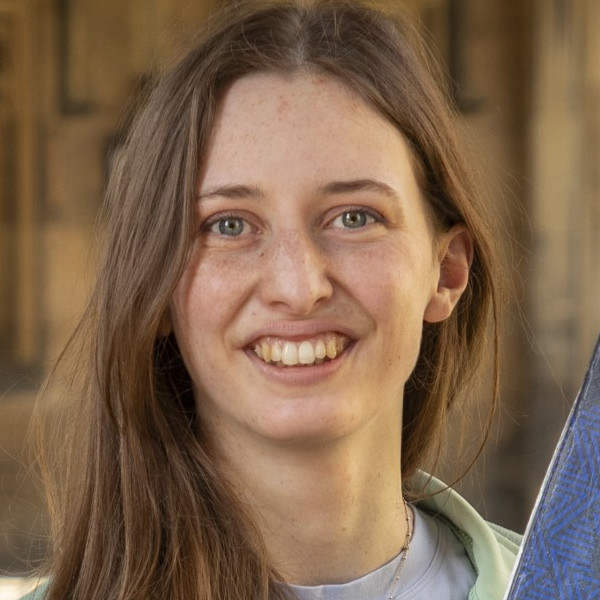
\includegraphics[width=0.09\textheight]{people/charlotte_priestley.jpg}%
        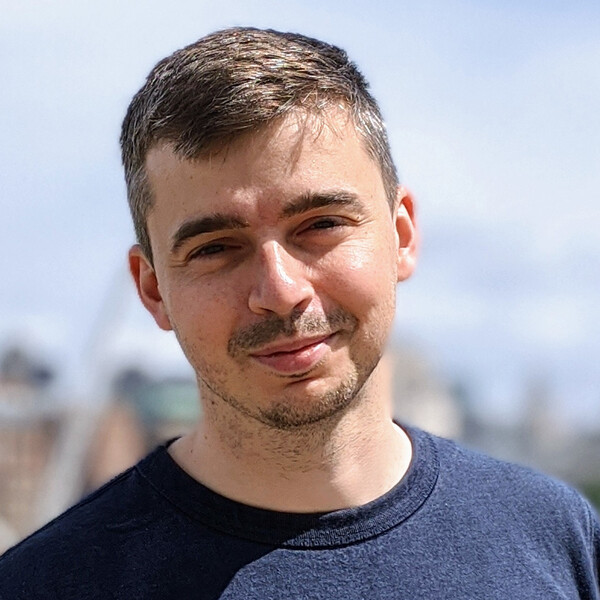
\includegraphics[width=0.09\textheight]{people/david_yallup.jpg}%
        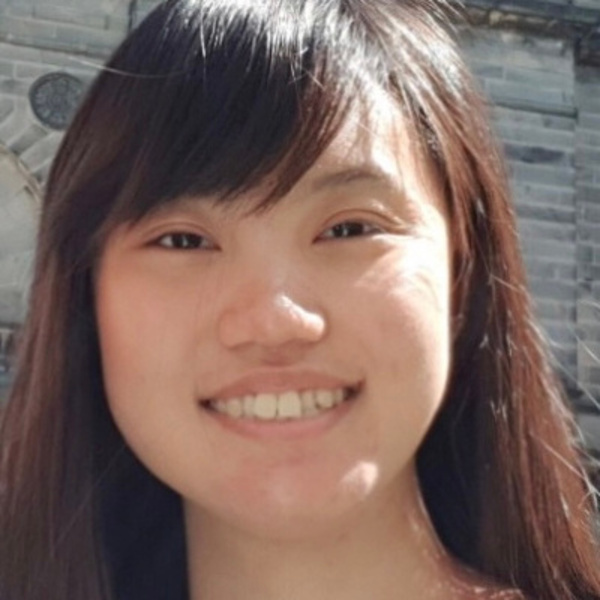
\includegraphics[width=0.09\textheight]{people/dily_ong.jpg}%
        
\includegraphics[width=0.09\textheight]{people/harry_bevins.jpg}%
        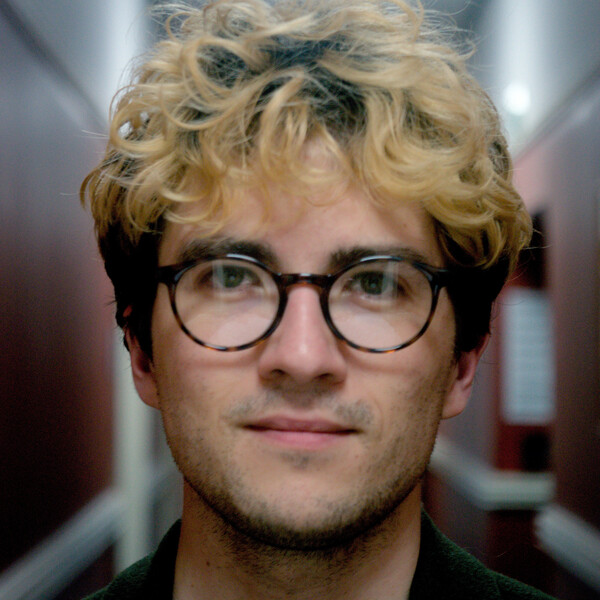
\includegraphics[width=0.09\textheight]{people/harvey_williams.jpg}%
        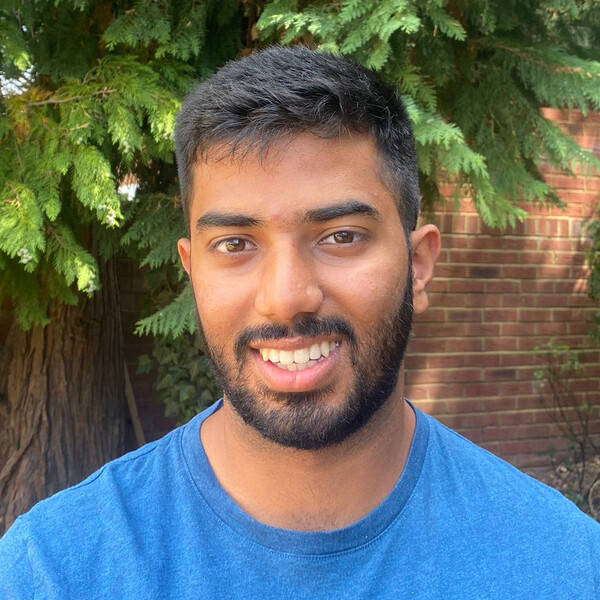
\includegraphics[width=0.09\textheight]{people/krish_nanavati.jpg}%
        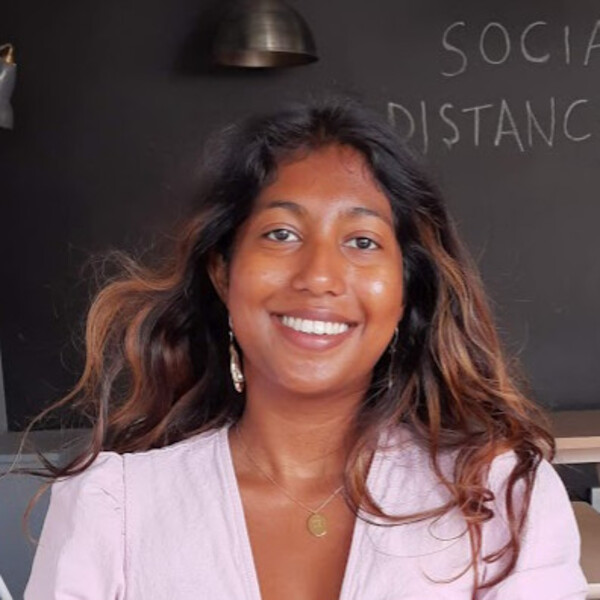
\includegraphics[width=0.09\textheight]{people/metha_prathaban.jpg}%
        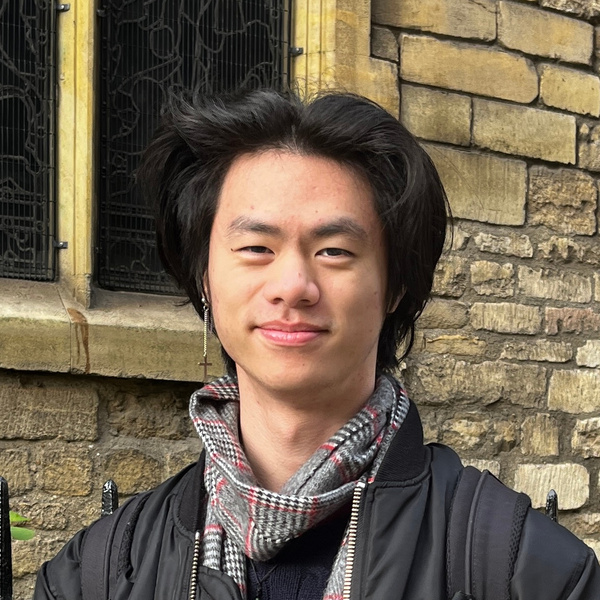
\includegraphics[width=0.09\textheight]{people/ming_yang.jpg}%
        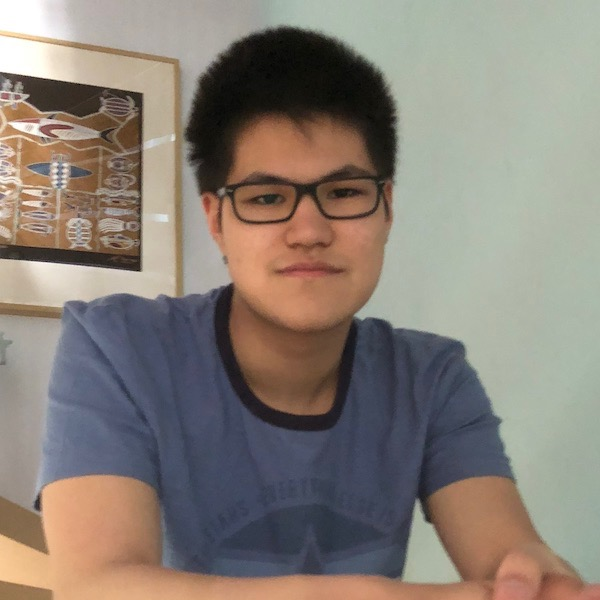
\includegraphics[width=0.09\textheight]{people/namu_kroupa.jpg}%
        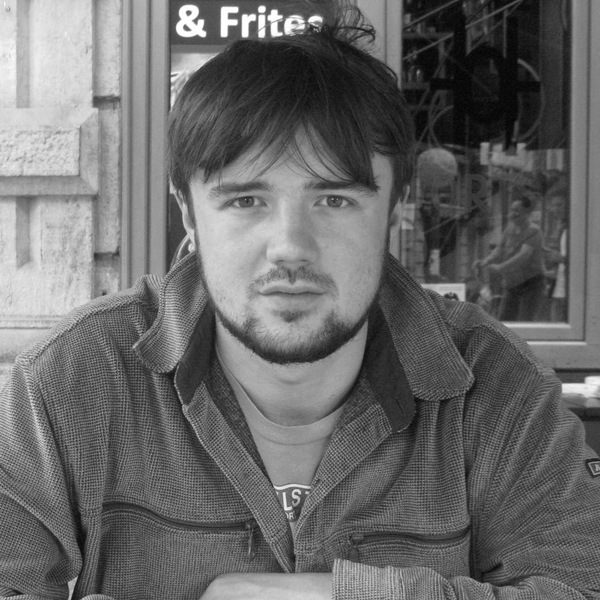
\includegraphics[width=0.09\textheight]{people/sam_leeney.jpg}%
        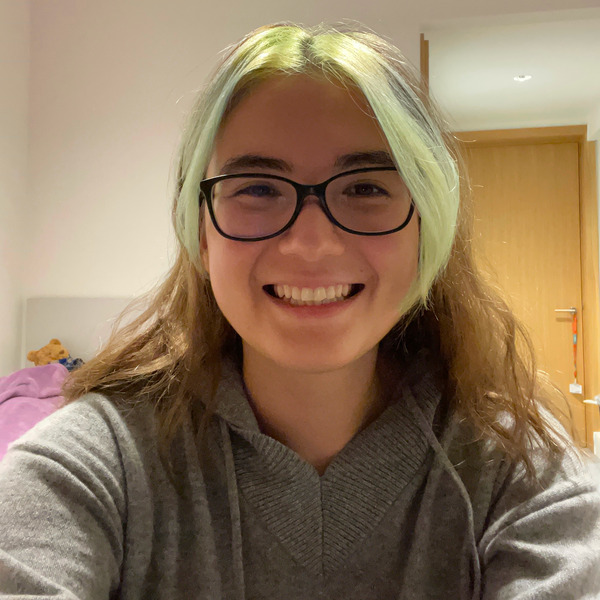
\includegraphics[width=0.09\textheight]{people/sinah_legner.jpg}%
        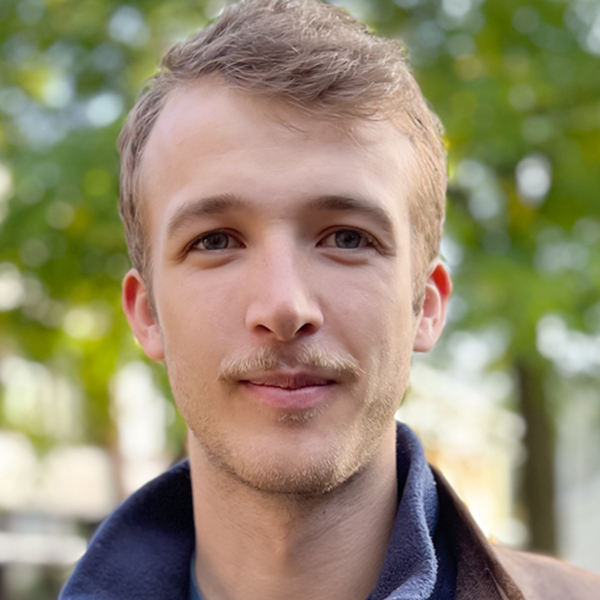
\includegraphics[width=0.09\textheight]{people/toby_lovick.jpg}%
        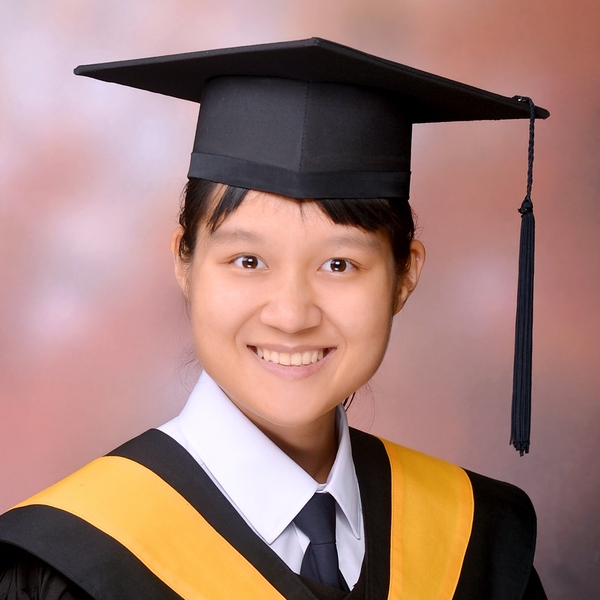
\includegraphics[width=0.09\textheight]{people/wei-ning_deng.jpg}%
        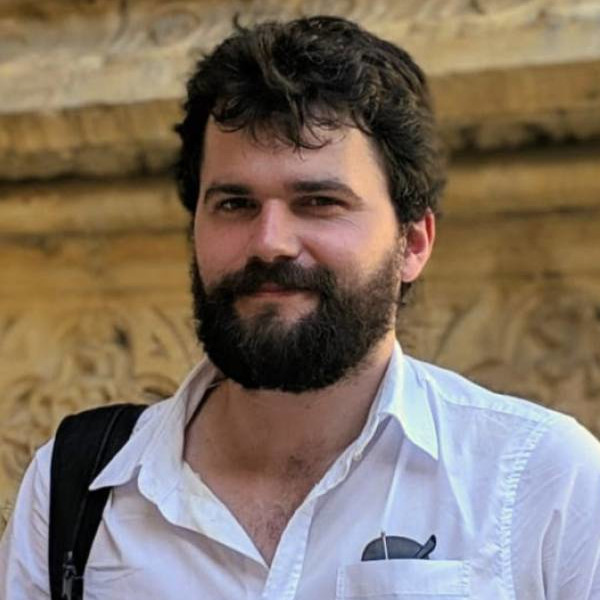
\includegraphics[width=0.09\textheight]{people/will_handley.jpg}%
        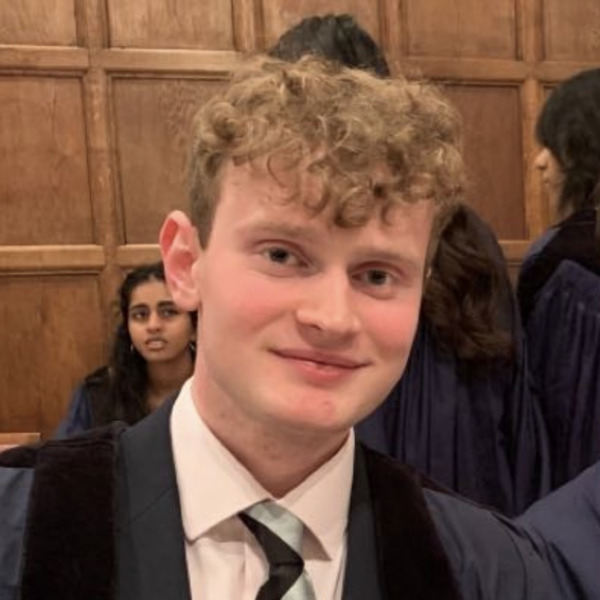
\includegraphics[width=0.09\textheight]{people/will_templeton.jpg}%
    };
\end{frame}

\end{document}
